\chapter{Implementation and Results} \label{ch:implementation}
The smartphone-based quadrotor control system developed in this project, is subjected to flight tests. the results of which are shown in this chapter. This chapter describes the Android application developed for the execution of the flight controller, detailing its activities and functions. In order to build a complete UAS, a GCS is developed and a communication channel is established between the Android application executed on board, and the desktop application (GCS). The quadrotor is tested for each designed flight mode and controller.
\\\\
In Section \ref{sec:app}, the flight control application, developed to run on the Android operating system, is detailed. Here, the activities of which the application is composed, and its functions, are detailed.
\\\\
The components and features of the GCS, are shown in Section \ref{sec:gcs}. This section details the characteristics of the developed desktop application, in addition to the communication channel established with the Android application, and therefore with the quadrotor. Finally, in Section \ref{sec:tests}, the results obtained after the execution of the flight tests in the quadrotor, are presented. These results show the quadrotor performance after being subjected to disturbances and changes of references, while executing the designed control and estimation algorithms.

\section{Android Application} \label{sec:app}
The flight controller application, designed for being executed in an Android smartphone, is exposed in this section. The application is based on nine activities, which allow the user to perform tests and data acquisition with or without being connected to the smartphone-to-ESC gateway. The application activities composition and its navigation flow, are shown in Fig. \ref{fig:mainActivities}.
\begin{figure}[H]
\begin{center}
\includegraphics[height=\textheight]{mainActivities}  
\caption{Activities diagram in the Android application} 
\label{fig:mainActivities}
\end{center}
\end{figure}
The activities description, based on the navigation flow shown in Fig. \ref{fig:mainActivities}, is detailed below.

\subsubsection{Launch Activity}
The launch activity is the activity executed first when starting the application. This activity is executed for around 3 seconds. Here, the initial load of the application is completed, and the required permissions are requested. These are the location and storage permissions.

\subsubsection{Main Activity}
This activity is the main interface of the application. From here, the user can access the mission, tests and information activities, as well as change application settings. If the interface does not receive any command, and the screen is not touched after 10 seconds of execution, the mission activity is executed automatically.

\subsubsection{Mission Activity}
The mission activity is the activity responsible for the execution of the flight controller. During the execution of this activity, a TCP server is created, which waits for the remote connection of the GCS. Additionally, the sensors of the smartphone, and the control and estimation algorithms, are initialized and are available to the flight controller. 
\\\\
Once the communication channel with the GCS is established, the flight controller initiates the decoding of frames coming from the GCS, which include commands of: arming or disarming of motors, flight mode change, waypoints setting, references changes, remote controller commands, and quadrotor data query.
\\\\
For debug purposes, the mission activity also has an interface that shows the flight mode in which the quadrotor is located, the current type of controller being executed, the status of the motors, current position and attitude, level of the smartphone and quadrotor batteries, number of received waypoints, and remote control commands. Also, the communication between the smartphone and the gateway can be tested using the button `Led On/Off', which sends a command to turn on or off the built-in led of the Arduino Mega ADK.


\subsubsection{Information Activity}
This activity shows information about this project and its author, so that the user of the application knows its origin.

\subsubsection{Tests Activity}
The preliminary tests of the smartphone-based quadrotor system can be accessed from this activity. These tests are: the communication test, position sensing test, attitude estimation test, and quadrotor motors test.

\subsubsection{Communication Test Activity}
The communication test activity allows the user to check if the communication channel between the Android application and the GCS, is working. Here, the user can turn on or off the TCP server, and watch some commands sent by the remote controller, through the GCS. 

\subsubsection{Position Test Activity}
The position test activity initializes the smartphone GNSS receiver and starts the GNSS data acquisition. This activity shows the raw GNSS data and its projection to the Magna-Sirgas coordinate system, in addition to the altitude value acquired from the barometer and the attitude from the rotation virtual sensor.

\subsubsection{Attitude Test Activity}
This activity shows the data obtained from the virtual rotation sensor, as well as the raw position of the GNSS, to the user. It also allows the simultaneous plot of two of these signals, which can be changed during the acquisition execution.

\subsubsection{Motors Test Activity}
Finally, the motors test activity allows the user to test the established communication between the smartphone and the Arduino Mega ADK. In this activity, the user can configure the \textit{PWM} signal sent to each motor separately, in addition to checking the status of the quadrotor and smartphone batteries. The motors thrust and torque tests, shown in Section \ref{sec:parameters}, are developed using this activity to command the motors thrust.

\section{Ground Control Station (GCS)}\label{sec:gcs}
The GCS is the land-based control station that adds monitoring and remote control functions for a UAV. For this project, the GCS software is designed using the Java programming language. The Java language is chosen in order to add portability to the application.
\\\\
As mentioned earlier, the Android application creates a TCP server in order to let the GCS, acting as a TCP client, exchange data packets with the smartphone. The communication between the Android application and the GCS, is based on a packet-based communication using the TCP and IP protocols. 
\\\\
The user can interact with the GCS through the mouse or touchscreen of the computer, or using a control for video games (remote controller) connected through the USB interface of the computer. Using button sequences commands through the remote controller, the user can establish and finish the connection with the quadrotor, change the flight mode, and arm or disarm the motors. Also, the quadrotor position and attitude references can be changed using the remote controller joysticks.
\\\\
The GCS interface, is composed by six main panels, shown in Fig. \ref{fig:missionGCS}, and a Communication tab, which are are described below.
\begin{figure}[h]
\begin{center}
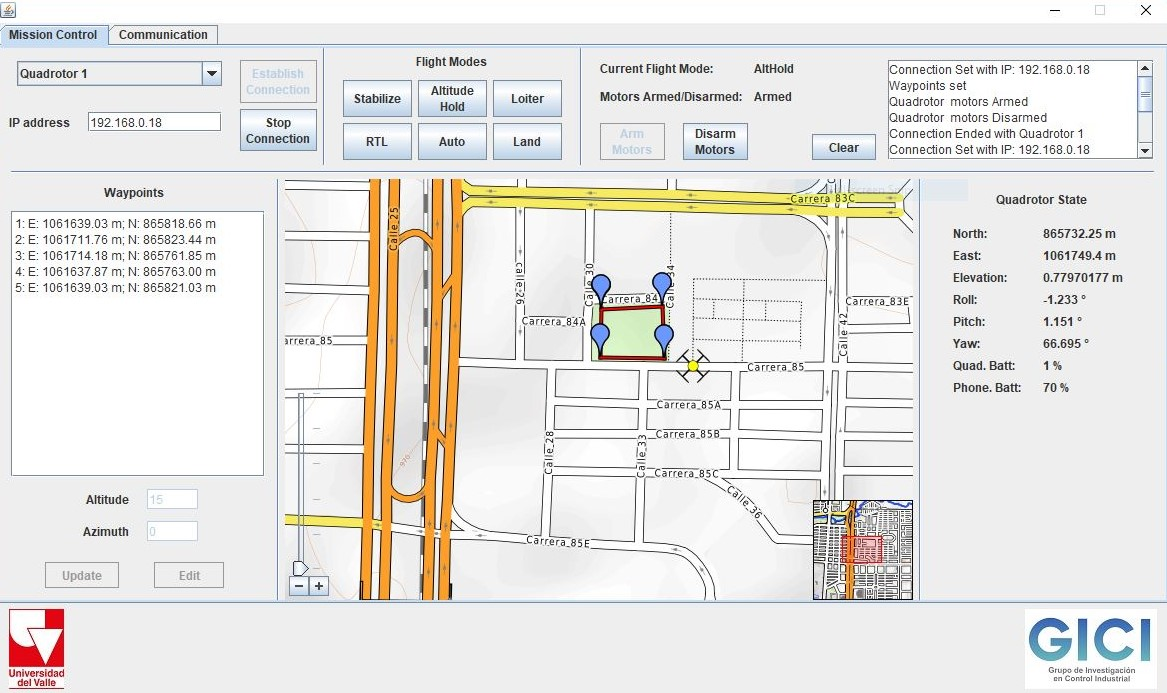
\includegraphics[width=\textwidth]{missionGCS.jpg}  
\caption{Ground Control System main interface} 
\label{fig:missionGCS}
\end{center}
\end{figure}

\subsubsection*{Connection Panel}
Located at the upper left edge of the GCS interface, this panel allows the user to select the quadrotor to which the user wants to connect and establish its IP address. This is the only panel enabled after the execution of the GCS. Once the connection with the quadrotor is established, the other panels are enabled.
\subsubsection*{Flight Modes Panel}
Once the connection is established, the user can select the desired flight mode using the buttons in the Flight Modes panel. After a flight mode button is pushed, the user is prompted to confirm its will to change the quadrotor flight mode. When a confirmation of flight mode change is received from the smartphone, the current flight mode, in the Status and Console Panel, is updated.
\subsubsection*{Status and Console Panel}
The Status and Console panel is located in the upper right edge of the GCS interface. This panel, shows the current status of the motors and flight mode. Additionally, this panel includes buttons for arming/disarming the quadrotor motors, and a console area. This console, show relevant information regarding the connection, waypoints, flight mode, and motors status.
\subsubsection*{Map Panel}
In order to check the current position of the quadrotor, a map is displayed in the Map Panel, located in the center of the GCS interface. This display is based on the JXMapViewer2 library and the Open Street Map (OSM) project. In the map, the user can select the waypoints that the quadrotor will visit, which will be automatically connected in the graph, and added to the waypoints list. Also, a quadrotor icon is displayed in the current geolocated position of the quadrotor so the user can track it. When the GCS has internet access, the map provider from OSM is set. Otherwise, the map is got from downloaded map tiles which are included in the GCS resources. The offline map is restricted to the area of the city of Cali, Colombia, while the online map is available for all the world. The map is projected using the Pseudo-Mercator projection.
\subsubsection*{Waypoints Panel}
The Waypoints panel is located on the left flank of the Map panel. This panel shows the list of waypoints dynamically, so it is updated each time a waypoint is added in the Map panel. Also, the waypoints coordinates can be edited by the user, and their position is automatically updated in the map.
\subsubsection*{Quadrotor State Panel}
The quadrotor state data is composed by the quadrotor position, the quadrotor attitude, the quadrotor battery level and the smartphone battery level. This data is shown in the Quadrotor State panel, located on the right of the Map panel. The quadrotor state values are updated each $100\ ms$.
\subsubsection*{Communication Tab}
Additionally, the GCS interface have a Communication tab, which includes a Controller Settings Panel shown in Fig. \ref{fig:commGCS}. This panel shows the connection status of the GCS with the remote controller. Also, it presents the current value of the remote controller joysticks and its buttons state.
\begin{figure}[h]
\begin{center}
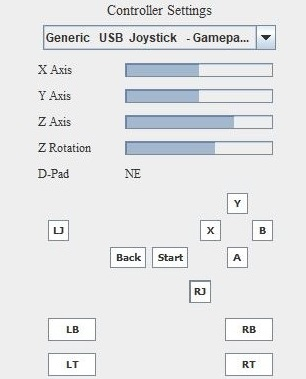
\includegraphics[width=0.3\textwidth]{commGCS.jpg}  
\caption{Controller settings in GCS} 
\label{fig:commGCS}
\end{center}
\end{figure}
\\\\
In order to obtain a wide range of wireless communication between the Android application and the GCS, an external high-gain WLAN antenna is used. Using this antenna, the quadrotor was tested to fly $200$ meters from the GCS with line of sight, without failing to keep a constant communication with the GCS.
\\\\
The complete UAS built in this project is shown in Fig. \ref{fig:UAS}. This UAS is composed by a smartphone-based quadrotor UAV, a GCS executing a java application for monitoring and remote control, and a WLAN-based communication channel between both of them.
\begin{figure}[h]
\begin{center}
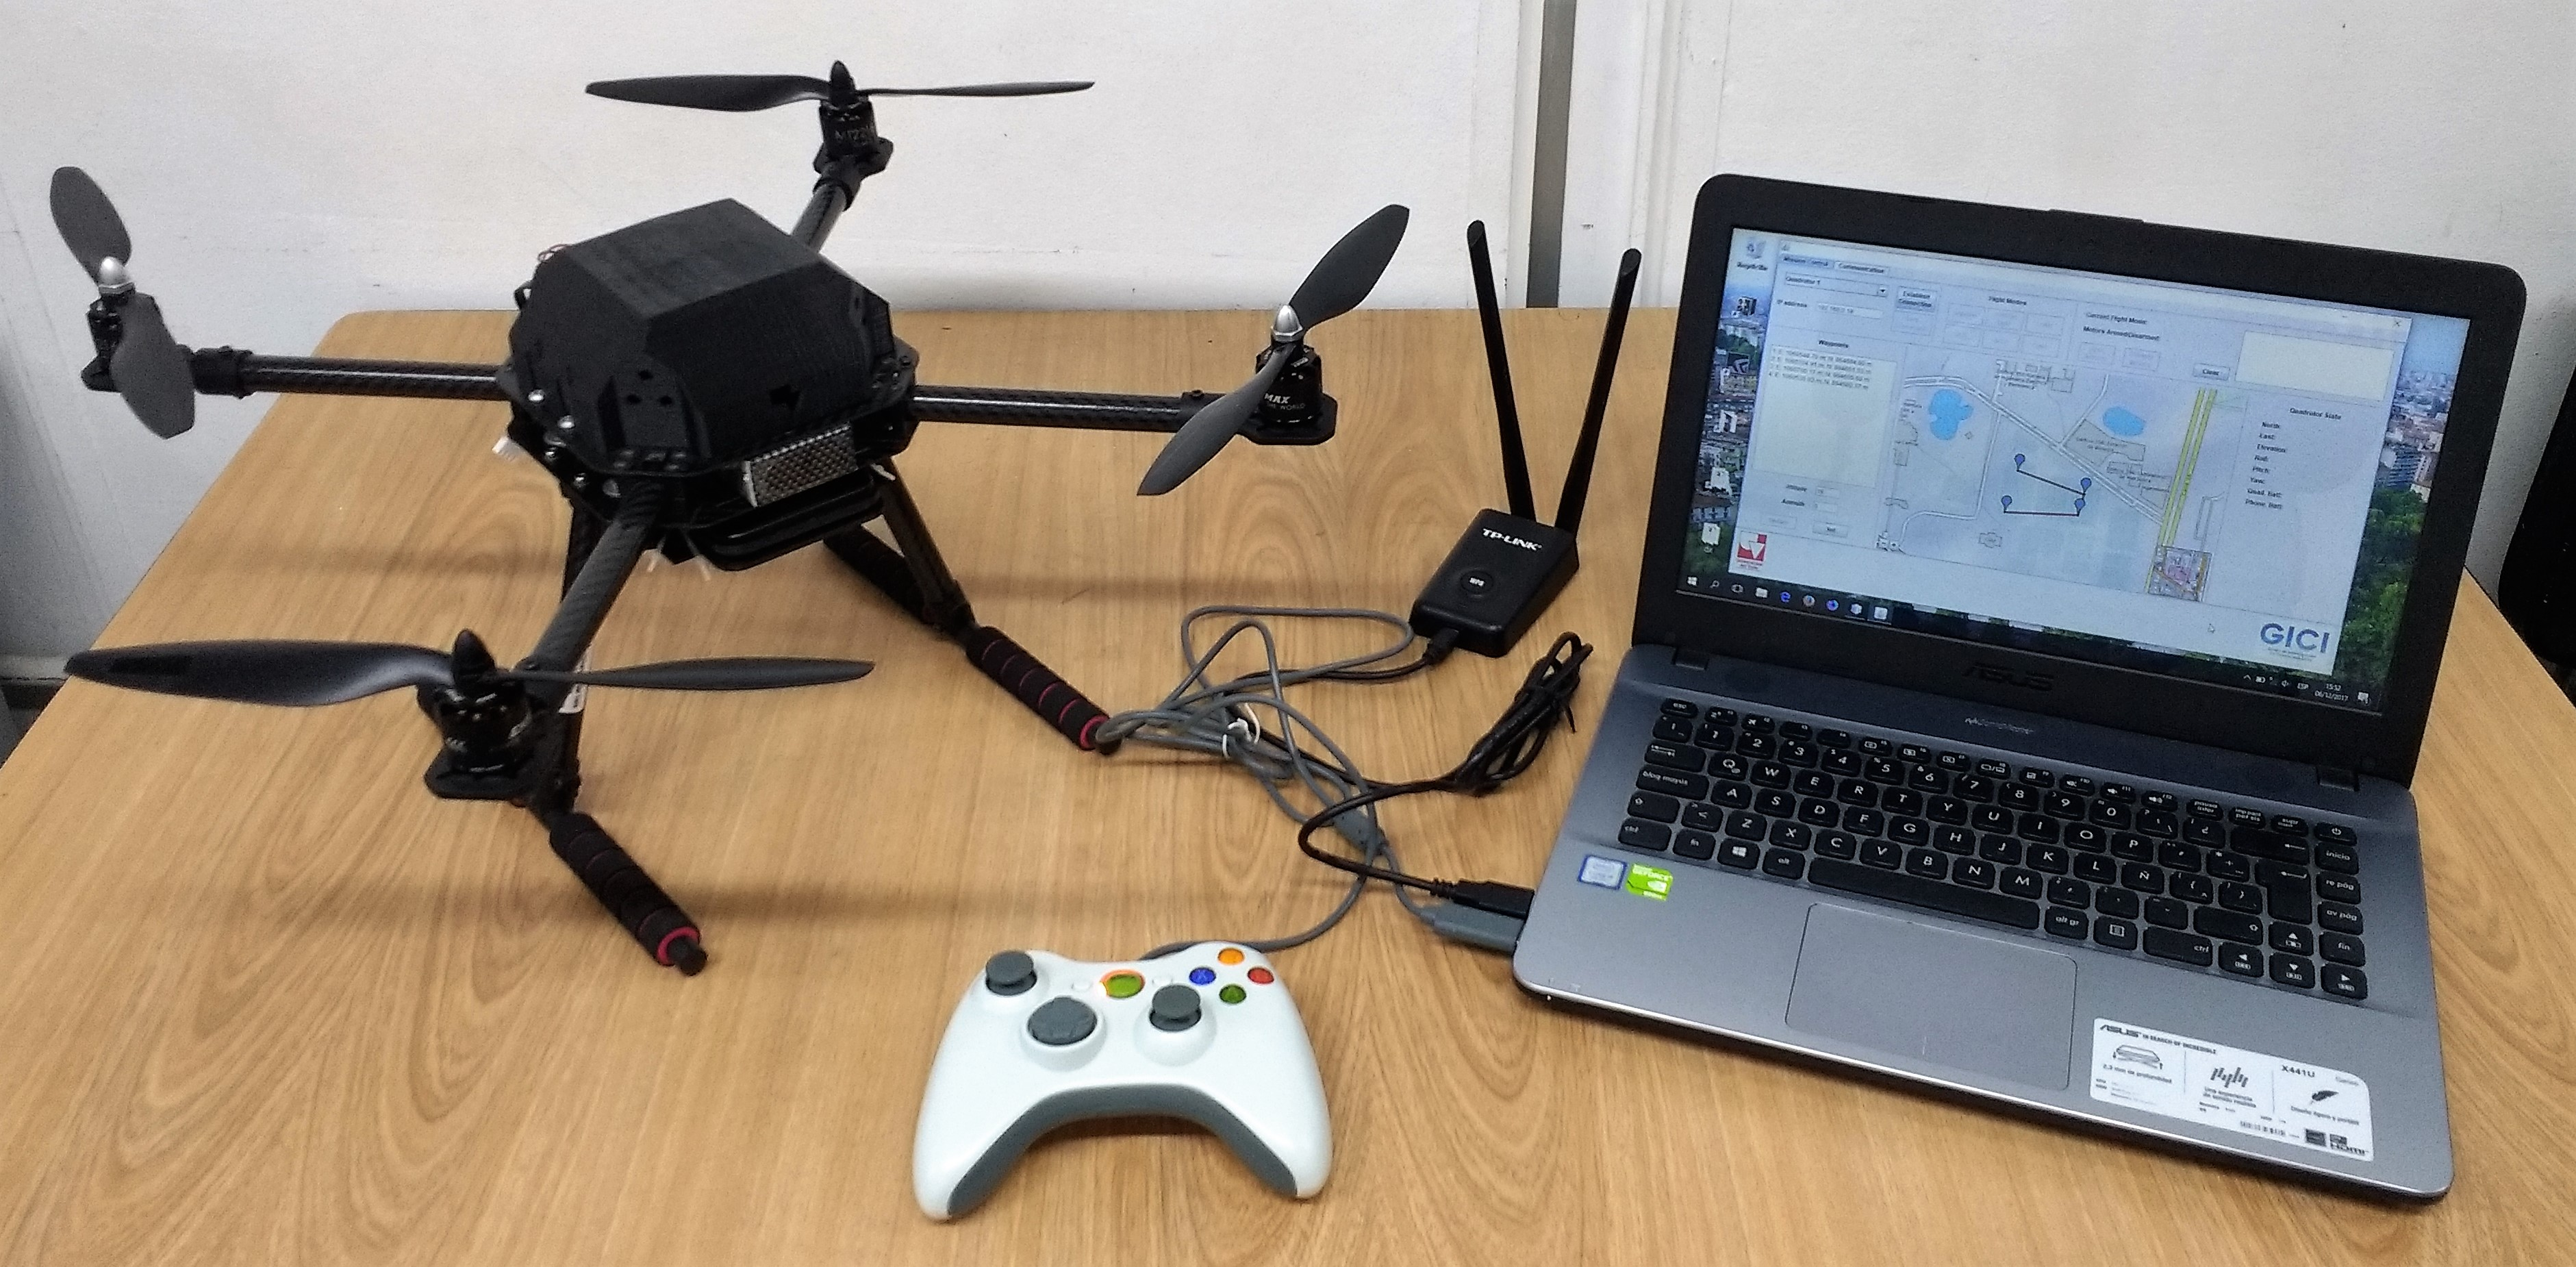
\includegraphics[width=0.75\textwidth]{UAS.jpg}  
\caption{Complete implemented Smartphone-based UAS} 
\label{fig:UAS}
\end{center}
\end{figure}

\section{Flight Tests} \label{sec:tests}
The control and estimation algorithms designed in Chapter \ref{ch:controlandestimation}, are implemented in the Android application that is executed in the smartphone on board the quadrotor. Using the smartphone-based quadrotor, the controllers are tested subjecting the system to disturbances and reference changes, within their flight modes. The results of these tests are shown in this section. The control signals $\mathbf{U} = \begin{bmatrix}
T_u & \tau_\psi & \tau_\theta & \tau_\phi
\end{bmatrix}^{T}$, and the \textit{PWM} signals, logged during each of the tests, are shown in Appendix \ref{controlsignals}.

\subsection{Stabilize Mode}
The smartphone-based quadrotor, in its stabilizing flight mode, is subjected to tests, in which a test bench based on a tripod and a ball head is used. The stabilize mode test bench, shown in Fig. \ref{fig:tripod}, was designed and built within the framework of this project. This test bench allows only rotational movements of the quadrotor, blocking its translational movements.
\begin{figure}[h]
\begin{center}
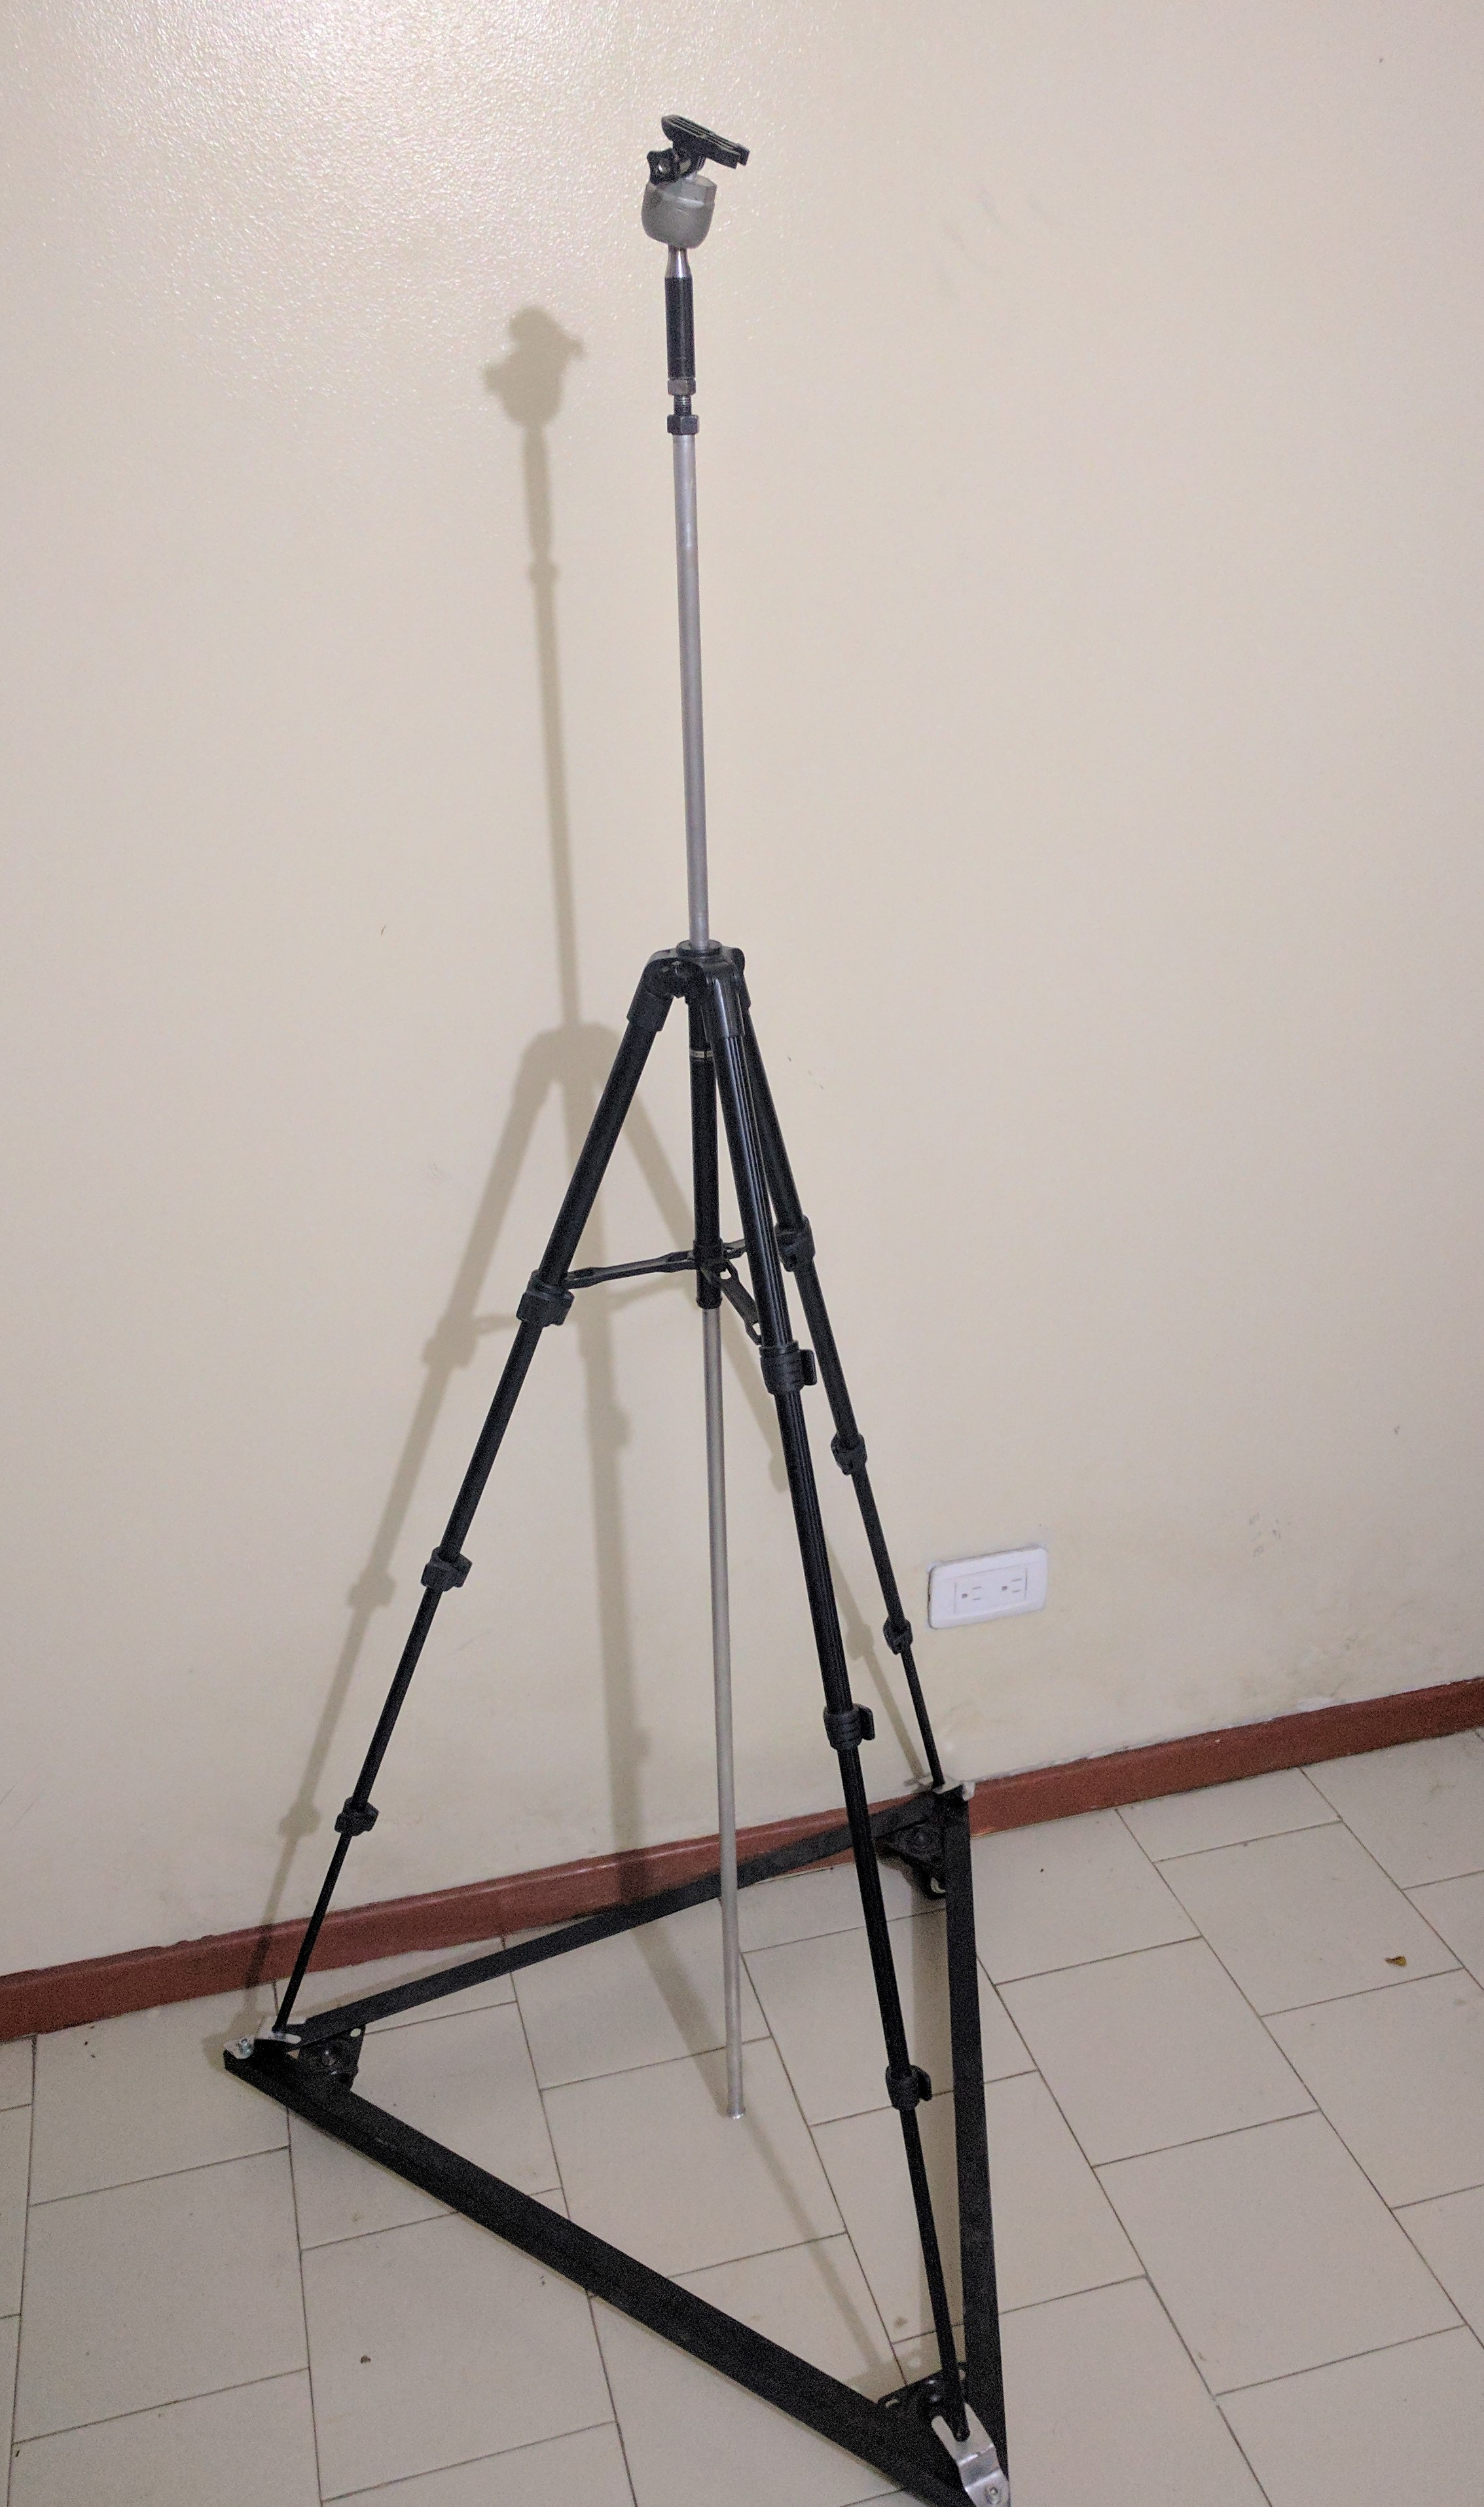
\includegraphics[width=0.3\textwidth]{tripod.jpg}  
\caption{Stabilize mode test bench} 
\label{fig:tripod}
\end{center}
\end{figure}

\subsubsection{LQI Controller}
The LQI controller in stabilize mode was tested by manually applying disturbances in the form of torques about the $x$, $y$ and $z$ axes, and successive reference changes from the remote controller.
\begin{figure}[H]
\begin{subfigure}{.5\linewidth}
\centering
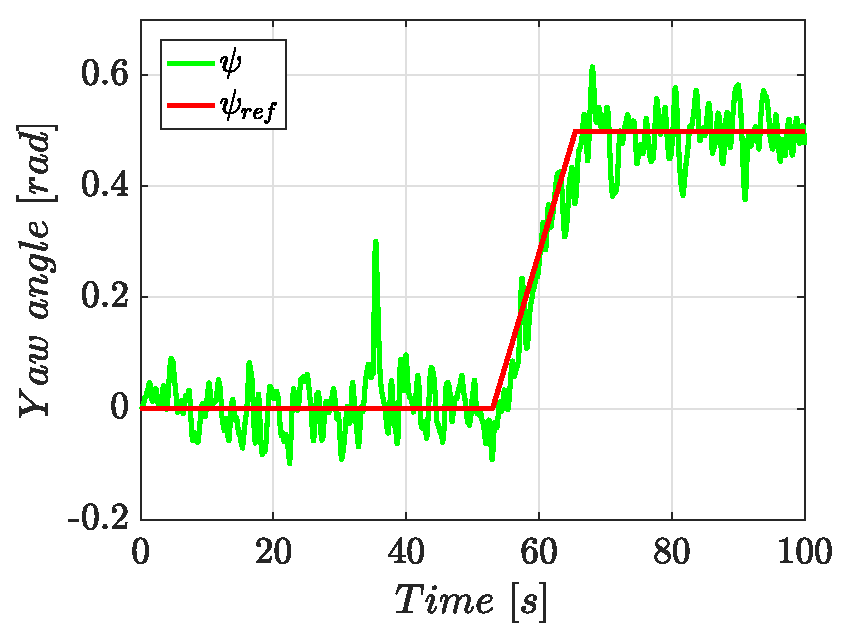
\includegraphics[width=7.0cm]{stabilize_psi_lqi_imp}
\caption{Yaw angle response}
\label{fig:stabilize_psi_lqi_imp}
\end{subfigure}%
\begin{subfigure}{.5\linewidth}
\centering
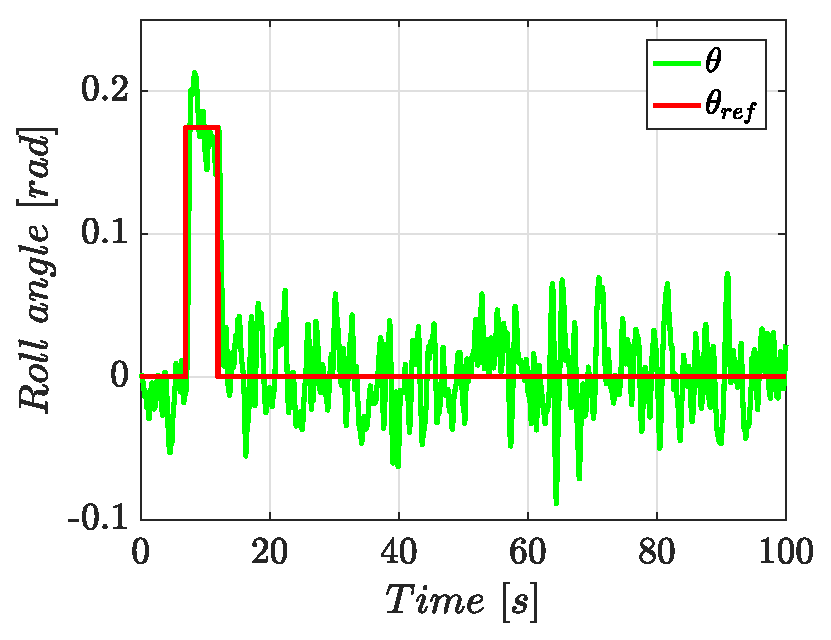
\includegraphics[width=7.0cm]{stabilize_theta_lqi_imp}
\caption{Roll angle response}
\label{fig:stabilize_theta_lqi_imp}
\end{subfigure}\\[1ex]
\begin{subfigure}{\linewidth}
\centering
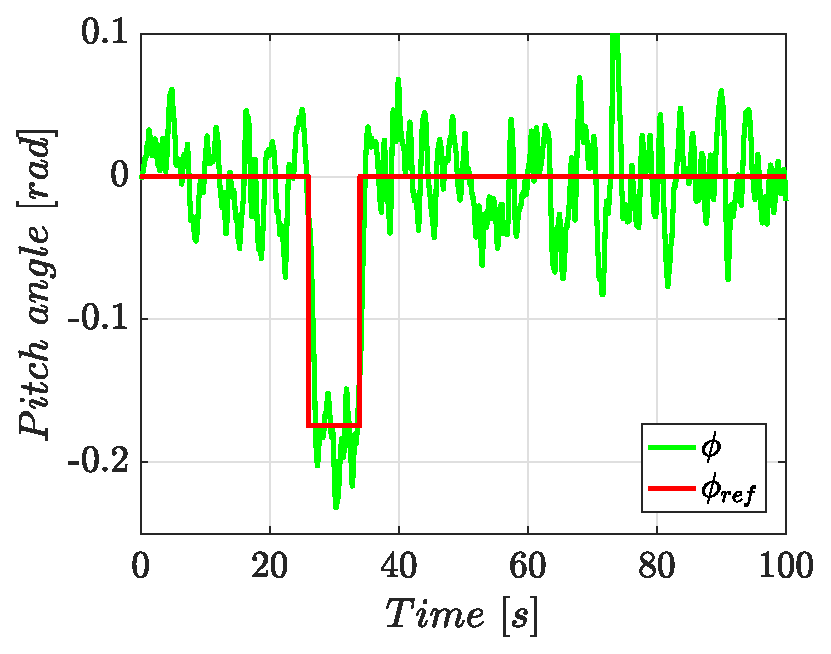
\includegraphics[width=7.0cm]{stabilize_phi_lqi_imp}
\caption{Pitch angle response}
\label{fig:stabilize_psi_lqi_imp}
\end{subfigure}
\caption{Closed-loop response of stabilize mode controlled by a LQI controller}
\label{fig:stabilize_lqi_imp}
\end{figure}
In Fig. \ref{fig:stabilize_lqi_imp}, the quadrotor response to the tests in stabilize mode, is shown. The yaw angle $\psi$ is subjected to a disturbance at $t = 34\ s$, and a slow reference change between $t = 53\ s$, to $t = 64\ s$. In the case of the roll angle $\theta$, the reference change is done momentarily, after $t = 8\ s$, and a disturbance is applied at $t = 67\ s$. On the other hand, at $t = 72\ s$, a disturbance in the torque $\tau_\phi$ is applied, and at $t = 24\ s$ the pitch angle $\phi$ reference is changed.

\subsubsection{$H_\infty$ Controller}
The same test, as with the LQI controller, is developed with the $H_\infty$ controller.
\begin{figure}[H]
\begin{subfigure}{.5\linewidth}
\centering
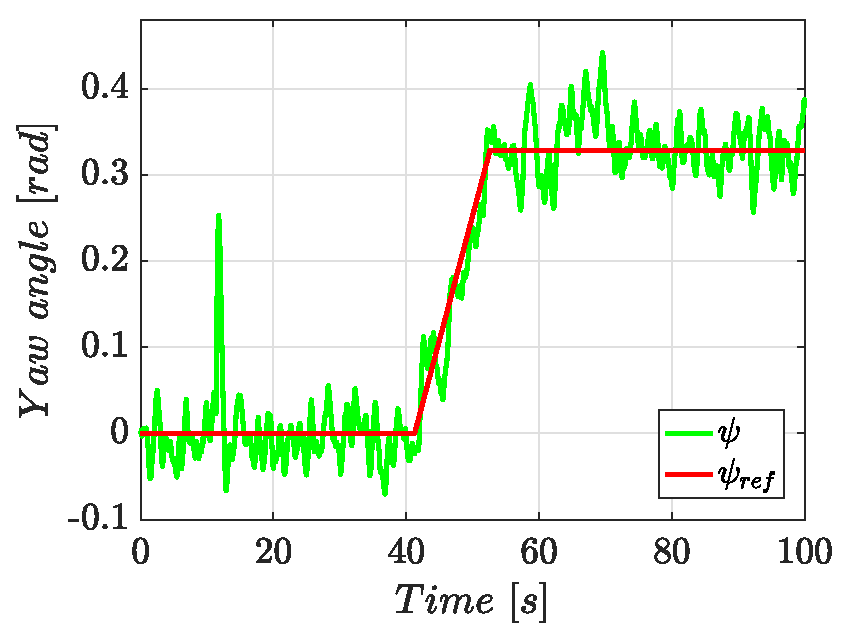
\includegraphics[width=7.0cm]{stabilize_psi_h_imp}
\caption{Yaw angle response}
\label{fig:stabilize_psi_h_imp}
\end{subfigure}%
\begin{subfigure}{.5\linewidth}
\centering
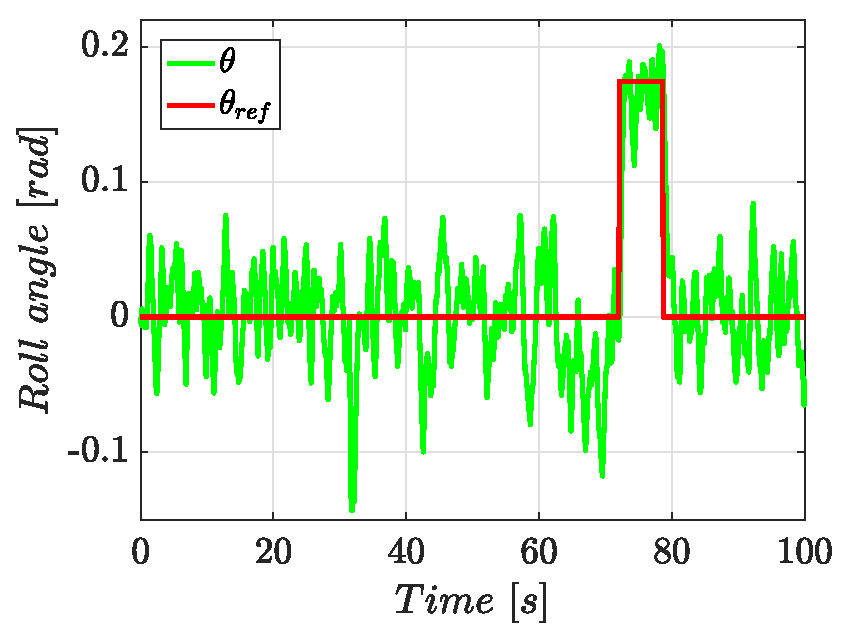
\includegraphics[width=7.0cm]{stabilize_theta_h_imp}
\caption{Roll angle response}
\label{fig:stabilize_theta_h_imp}
\end{subfigure}\\[1ex]
\begin{subfigure}{\linewidth}
\centering
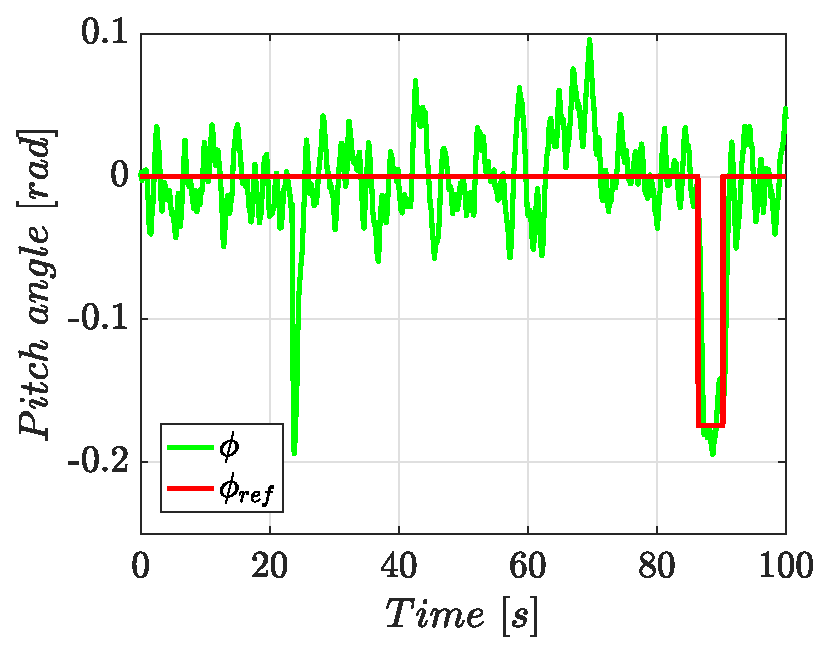
\includegraphics[width=7.0cm]{stabilize_phi_h_imp}
\caption{Pitch angle response}
\label{fig:stabilize_psi_h_imp}
\end{subfigure}
\caption{Closed-loop response of stabilize mode controlled by a $H_\infty$ controller}
\label{fig:stabilize_h_imp}
\end{figure}
In this case, as seen in Fig. \ref{fig:stabilize_h_imp}, the disturbances are applied at $t = 11\ s$ for $\psi$, $t = 23\ s$ for $\phi$, and $t = 32\ s$ for $\theta$. However, the reference of $\psi$ is changed between $t = 41\ s$ and $t = 53\ s$, while the references change in $\theta$ and $\phi$ are applied at $t = 71\ s$ and $t = 86\ s$ respectively.

\subsubsection{Performance}
Both of the controllers were capable of stabilize the quadrotor attitude dynamics. For the stabilize mode tests, the performance of the controllers is evaluated taking into account the setting time and overshoot of the controlled signals. These indices are shown in Table \ref{tb:stabilize_index}.
\begin{table}[H]
\small
\begin{center}
\caption{Performance indices - Stabilize mode tests}\label{tb:stabilize_index}
\begin{tabular}{c|c|c|c}\hline
\rule{0pt}{3ex} Controller & Controlled variable & Setting time $[s]$ & Overshoot $[\%]$ \\\hline\hline
\rule{0pt}{3ex} 
\multirow{3}{*}{LQI} 
 & $\psi$ & $1.39$ & $10.52$ \\
 & $\theta$ & $1.16$ & $17.39$ \\
 & $\phi$ & $1.12$ & $13.81$\\ \hline
\multirow{3}{*}{$H_\infty$} 
 & $\psi$ & $1.18$ & $9.84$ \\
 & $\theta$ & $1.03$ & $8.40$ \\
 & $\phi$ & $1.29$ & $5.67$ \\ \hline\hline
\end{tabular}
\end{center}
\end{table}
The performance indices for the stabilize mode tests show that both the LQI and $H_\infty$ controllers designed for the stabilize flight mode, have similar setting time, but different overshoot percentage. The $H_\infty$ controller is the one with the lower overshoot and setting time, except for the setting time of the $\phi$ signal, which is lower when using the LQI controller.
\\\\
\subsection{Altitude Hold Mode}
The altitude flight mode tests were performed on a football field of the Universidad del Valle. This place was chosen because it is an open space free of obstacles, where the quadrotor has total freedom to move without being at risk of colliding with something or somebody.
\\\\
In these tests, the only variable that was intentionally affected was the quadrotor altitude $z$. Hence, the references regarding the roll, pitch and yaw angles, are left in zero during the tests.

\subsubsection{LQI Controller}
As seen in Fig. \ref{fig:althold_lqi_imp}, the quadrotor altitude reference was changed at $t = 33\ s$. A disturbance was applied by manually pulling the quadrotor down with a rope at $t = 42\ s$.
\begin{figure}[H]
\begin{subfigure}{.5\linewidth}
\centering
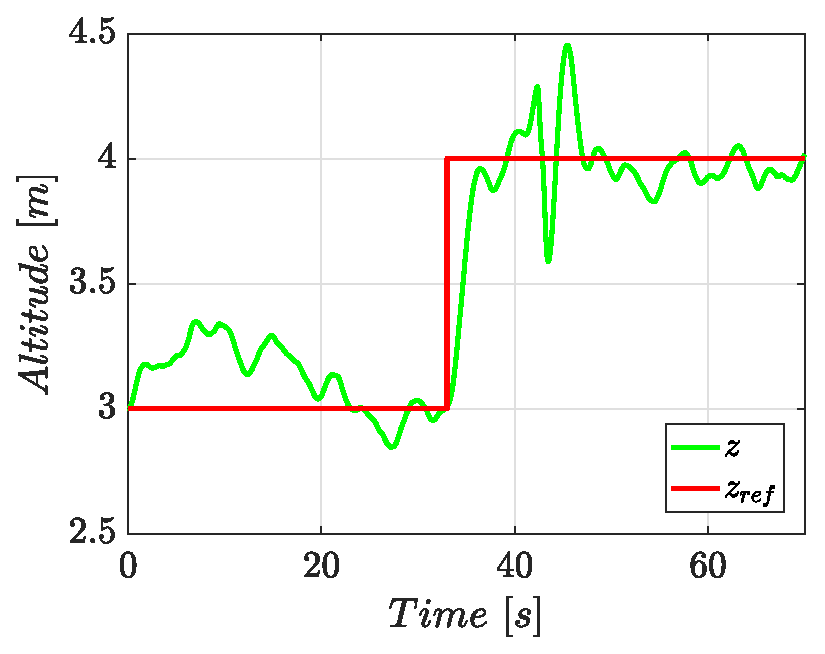
\includegraphics[width=7.0cm]{althold_z_lqi_imp}
\caption{$z$ position response}
\label{fig:althold_z_lqi_imp}
\end{subfigure}%
\begin{subfigure}{.5\linewidth}
\centering
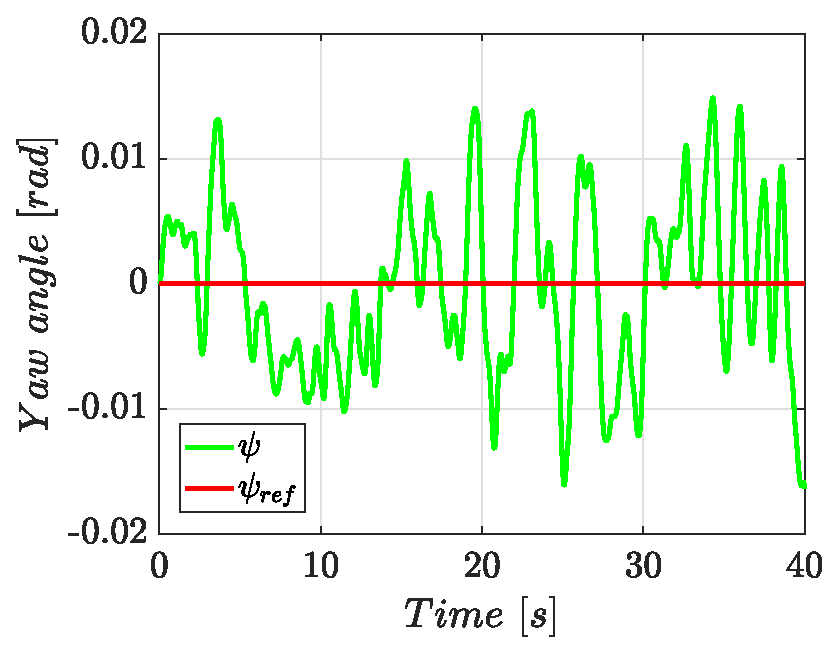
\includegraphics[width=7.0cm]{althold_psi_lqi_imp}
\caption{Yaw angle response}
\label{fig:althold_psi_lqi_imp}
\end{subfigure}\\[1ex]
\begin{subfigure}{0.5\linewidth}
\centering
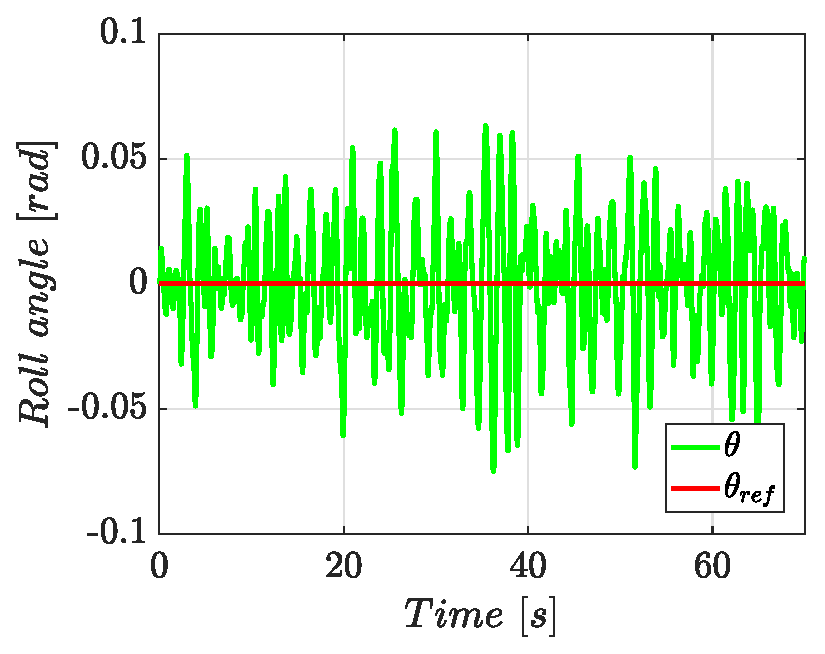
\includegraphics[width=7.0cm]{althold_theta_lqi_imp}
\caption{Roll angle response}
\label{fig:althold_theta_lqi_imp}
\end{subfigure}
\begin{subfigure}{0.5\linewidth}
\centering
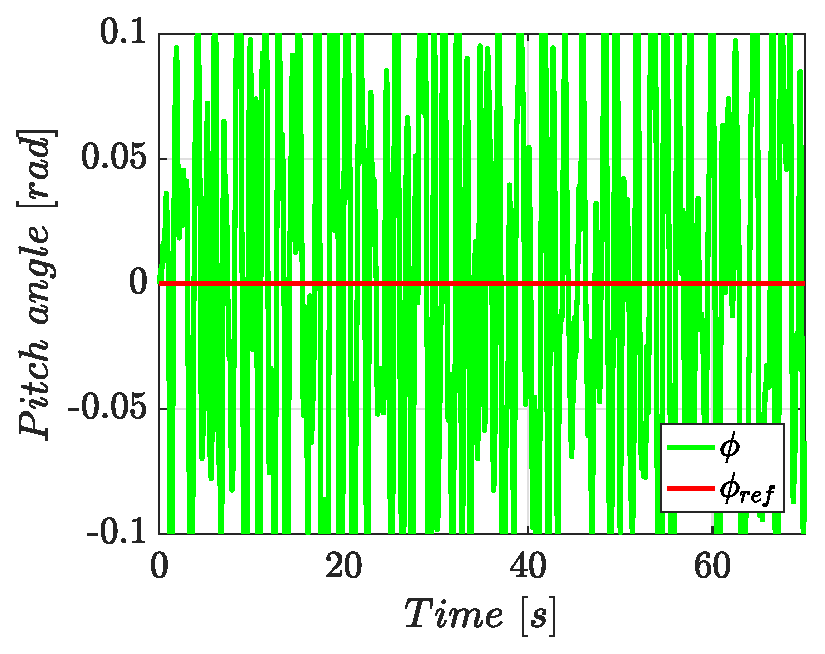
\includegraphics[width=7.0cm]{althold_phi_lqi_imp}
\caption{Pitch angle response}
\label{fig:althold_phi_lqi_imp}
\end{subfigure}
\caption{Closed-loop response of altitude hold mode controlled by a LQI controller}
\label{fig:althold_lqi_imp}
\end{figure}


\subsubsection{$H_\infty$ Controller}
Under approximately the same environmental conditions, the altitude hold mode test is developed with the $H_\infty$ controller being executed in the smartphone on board the quadrotor.
\\\\
In Fig. \ref{fig:althold_h_imp} is seen that the disturbance was applied, pulling the rope, at $t = 49\ s$, while the altitude reference was changed at $t = 42\ s$.
\begin{figure}[H]
\begin{subfigure}{.5\linewidth}
\centering
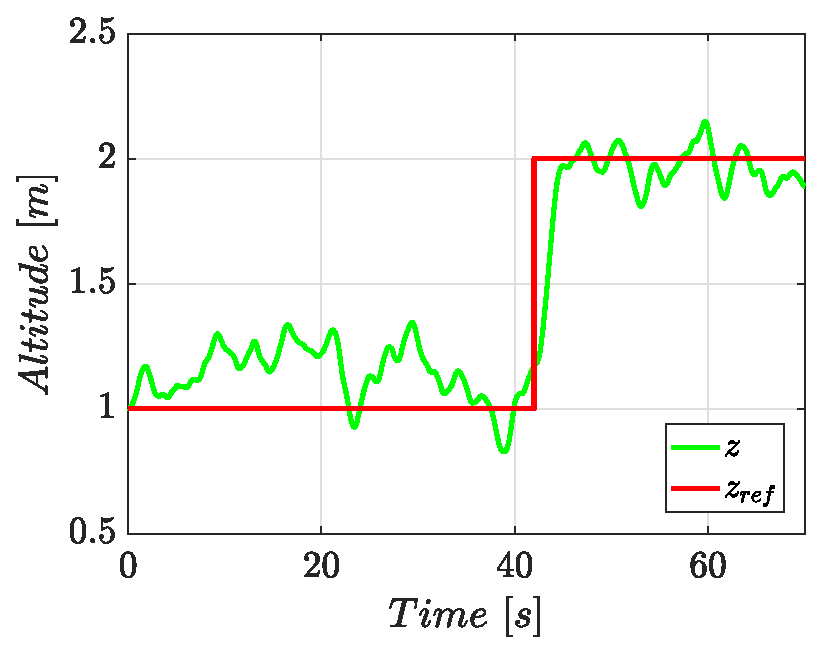
\includegraphics[width=7.0cm]{althold_z_h_imp}
\caption{$z$ position response}
\label{fig:althold_z_h_imp}
\end{subfigure}%
\begin{subfigure}{.5\linewidth}
\centering
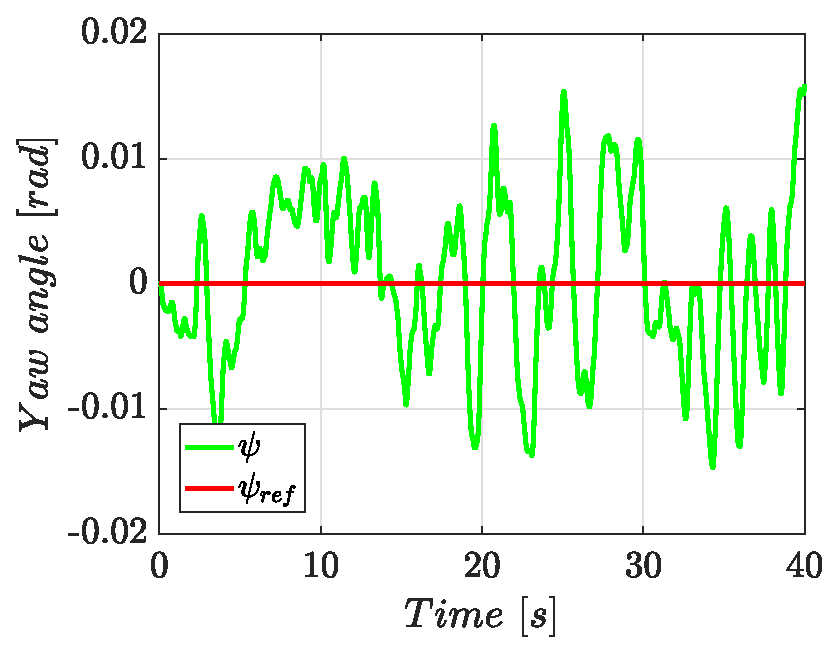
\includegraphics[width=7.0cm]{althold_psi_h_imp}
\caption{Yaw angle response}
\label{fig:althold_psi_h_imp}
\end{subfigure}\\[1ex]
\begin{subfigure}{0.5\linewidth}
\centering
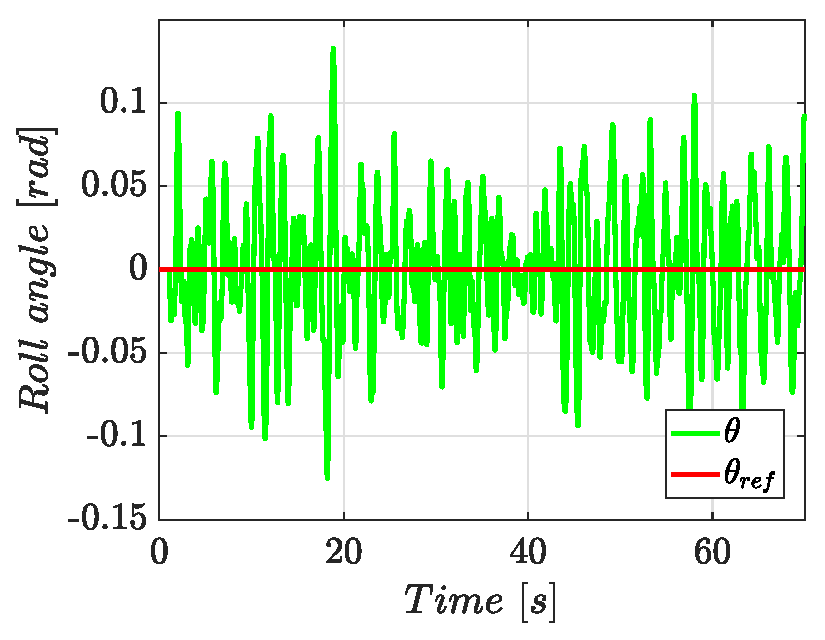
\includegraphics[width=7.0cm]{althold_theta_h_imp}
\caption{Roll angle response}
\label{fig:althold_theta_h_imp}
\end{subfigure}
\begin{subfigure}{0.5\linewidth}
\centering
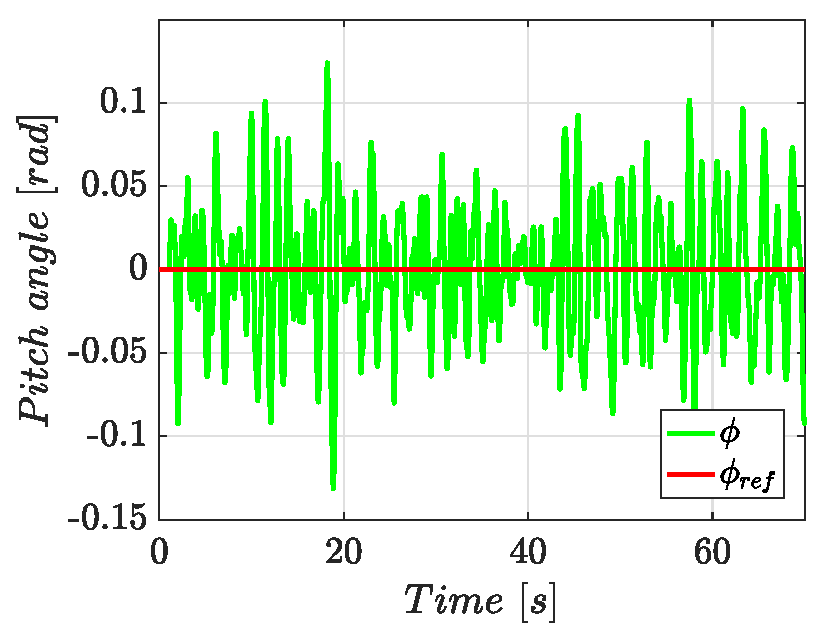
\includegraphics[width=7.0cm]{althold_phi_h_imp}
\caption{Pitch angle response}
\label{fig:althold_phi_h_imp}
\end{subfigure}
\caption{Closed-loop response of altitude hold mode controlled by a $H_\infty$ controller}
\label{fig:althold_h_imp}
\end{figure}

\subsubsection{Performance}
The quadrotor altitude control is achieved when implementing both the LQI and $H_\infty$ controllers.
The position error is calculated as the Euclidean distance between the quadrotor position and the reference position in each time step. The quadrotor achieves errors less than $0.4\ m$ during constant reference tracking, with both controllers. However, as shown in Fig. \ref{fig:althold_errorpos_imp}, during the reference change, the error is lower when executing the $H_\infty$ controller.
\\\\
In Table \ref{tb:althold_index}, the overshoot and setting time indices of the tests developed in the altitude hold mode, are shown. Regarding these indices, the $H_\infty$ controller presents slightly better results compared with the LQI controller.
\begin{figure}[hh]
\begin{subfigure}{.5\linewidth}
\centering
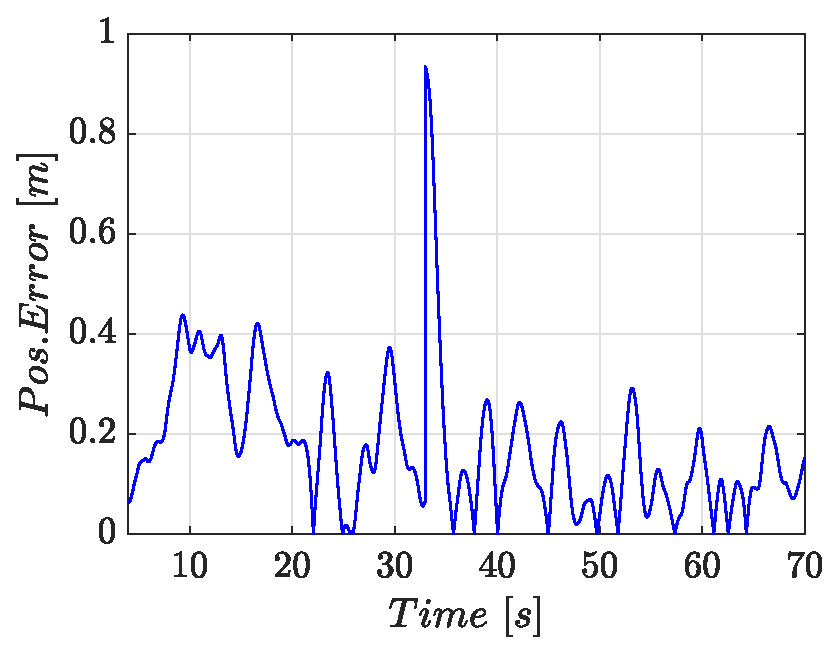
\includegraphics[width=7.0cm]{althold_errorpos_lqi_imp}
\caption{Position error with LQI controller}
\label{fig:althold_errorpos_lqi_imp}
\end{subfigure}%
\begin{subfigure}{.5\linewidth}
\centering
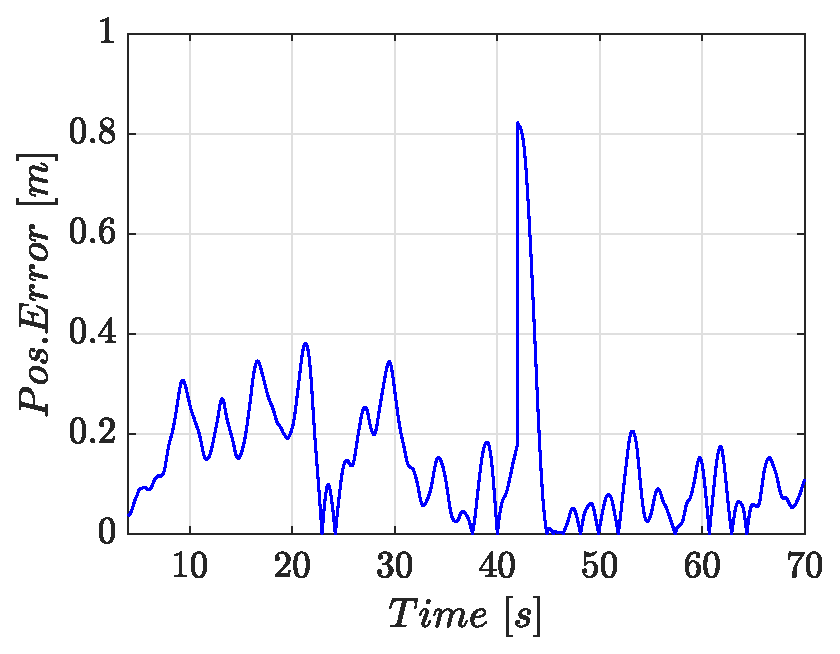
\includegraphics[width=7.0cm]{althold_errorpos_h_imp}
\caption{Position error with $H_\infty$ controller}
\label{fig:althold_errorpos_h_imp}
\end{subfigure}
\caption{Position errors in altitude hold mode}
\label{fig:althold_errorpos_imp}
\end{figure}
\begin{table}[h]
\small
\begin{center}
\caption{Performance indices - Altitude holde mode tests}\label{tb:althold_index}
\begin{tabular}{c|c|c|c}\hline
\rule{0pt}{3ex} Controller & Controlled variable & Setting time $[s]$ & Overshoot $[\%]$ \\\hline\hline
\rule{0pt}{3ex} 
\multirow{1}{*}{LQI} 
 & $z$ & $5.21$ & $8.71$ \\ \hline
\multirow{1}{*}{$H_\infty$} 
 & $z$ & $4.49$ & $5.36$ \\ \hline\hline
\end{tabular}
\end{center}
\end{table}
\\\\
\subsection{GNSS-Dependent Modes}
The tests regarding the GNSS-Dependent flight modes, are executed in the same scenario as the altitude hold mode tests. In this case, the variables of interest for the tests are the $ x $, $y $ and $ z $ positions.
\\\\
The references used in these tests are selected in a way that the same signal excursions as those used in Section \ref{sec:controldesign} are described. The performance of the controllers in the GNSS-Dependent modes is evaluated using the position error signal.

\subsubsection{LQI Controller}
This test was developed on the same soccer field as the altitude hold mode tests. During the execution of the test, there was no considerable presence of wind. In
Fig. \ref{fig:auto_xyz_lqi_imp}, the results of the LQI controller test for GNSS-Dependent modes, are shown. As detailed in Section \ref{sec:controldesign}, the reference trajectory describes a square of two meters on each side, with constant altitude.
\begin{figure}[h]
	\begin{center}
	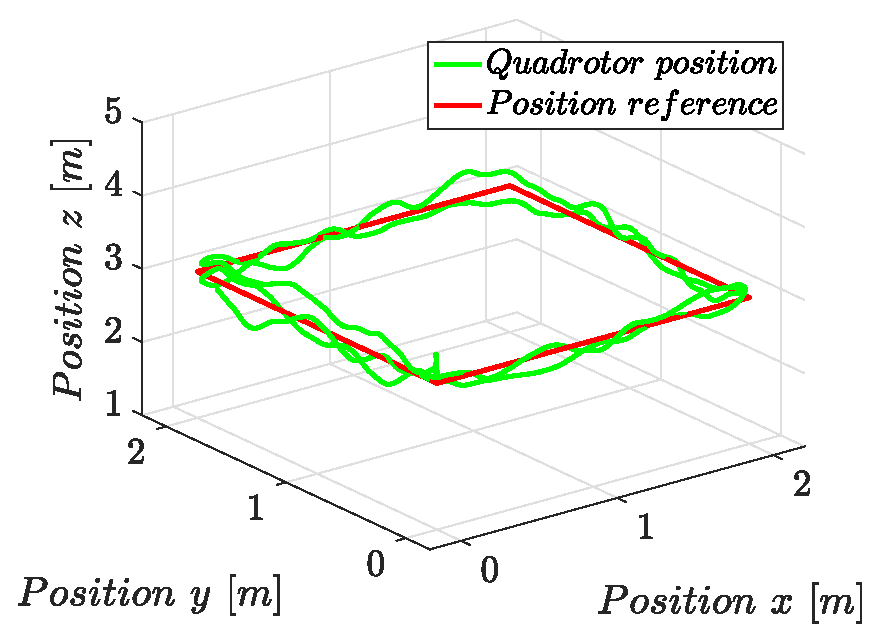
\includegraphics[width=0.7\textwidth]{auto_xyz_lqi_imp}
	\caption{Position response of the GNSS-Dependent modes with a LQI controller}
	\label{fig:auto_xyz_lqi_imp}
	\end{center}
	\end{figure}
	
%\begin{figure}[H]
%\begin{subfigure}{.5\linewidth}
%\centering
%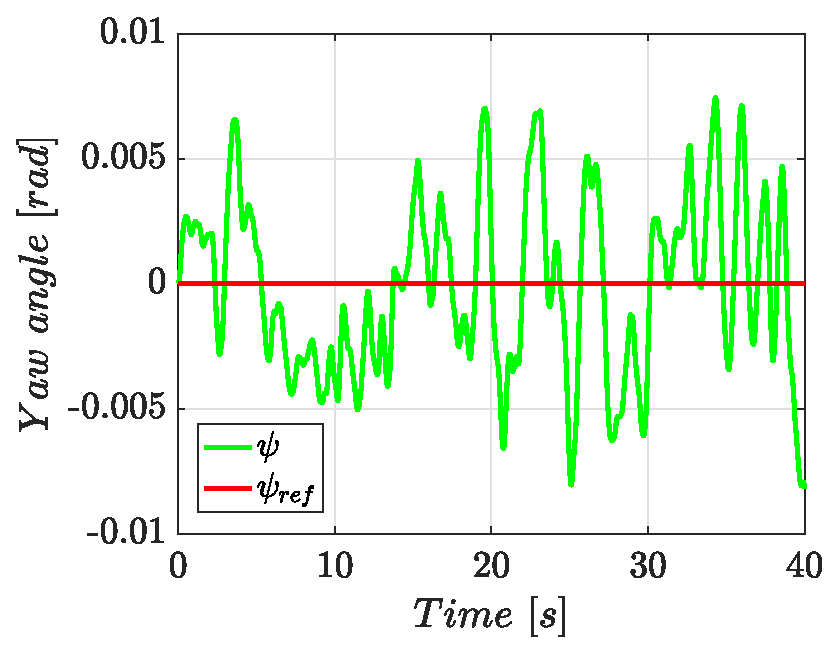
\includegraphics[width=7.0cm]{auto_psi_lqi_imp}
%\caption{Yaw angle response}
%\label{fig:auto_psi_lqi_imp}
%\end{subfigure}%
%\begin{subfigure}{.5\linewidth}
%\centering
%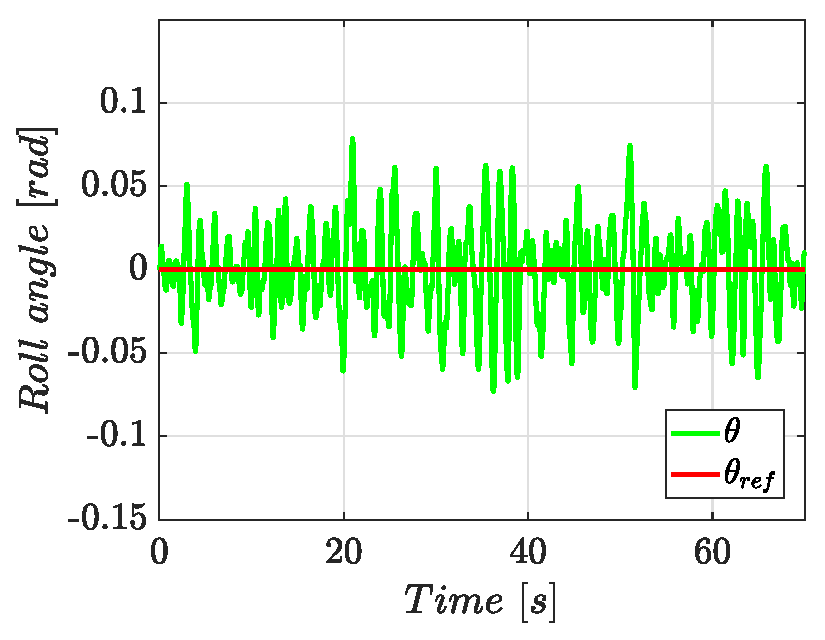
\includegraphics[width=7.0cm]{auto_theta_lqi_imp}
%\caption{Roll angle response}
%\label{fig:auto_theta_lqi_imp}
%\end{subfigure}\\[1ex]
%\begin{subfigure}{\linewidth}
%\centering
%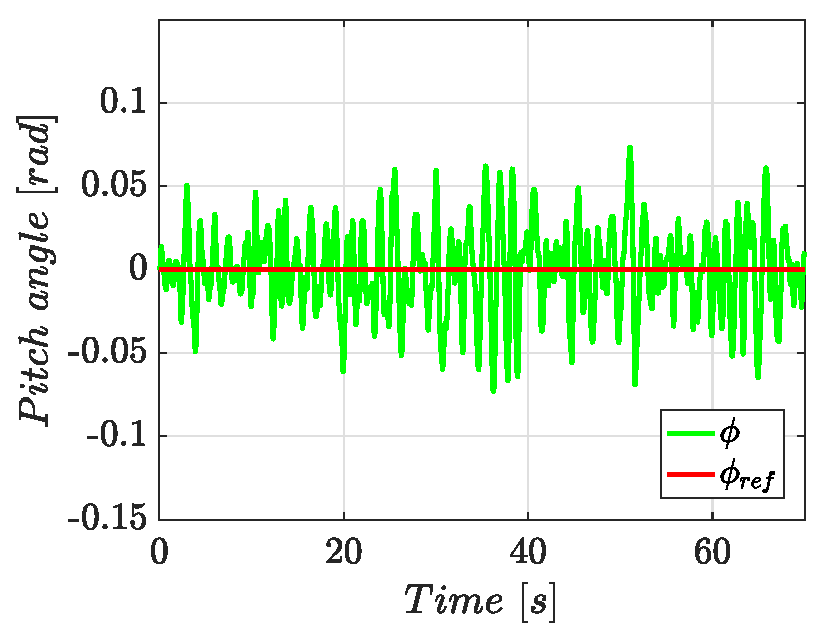
\includegraphics[width=7.0cm]{auto_phi_lqi_imp}
%\caption{Pitch angle response}
%\label{fig:auto_psi_lqi_imp}
%\end{subfigure}
%\caption{Attitude response of the GNSS-Dependent modes with a LQI controller}
%\label{fig:auto_lqi_imp}
%\end{figure}


\subsubsection{$H_\infty$ Controller}
The $H_\infty$ controller test, in GNSS-Dependent modes, was developed approximately $60$ minutes after the LQI controller test, with similar weather conditions.
\begin{figure}[h]
	\begin{center}
	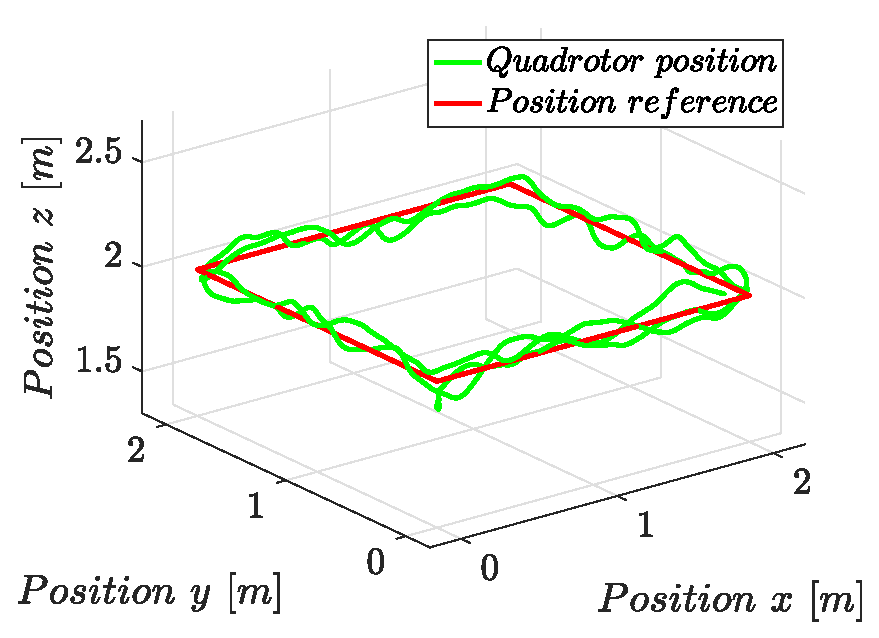
\includegraphics[width=0.7\textwidth]{auto_xyz_h_imp}
	\caption{Position response of the GNSS-Dependent modes with a $H_\infty$ controller}
	\label{fig:auto_xyz_h_imp}
	\end{center}
	\end{figure}
%	
%\begin{figure}[H]
%\begin{subfigure}{.5\linewidth}
%\centering
%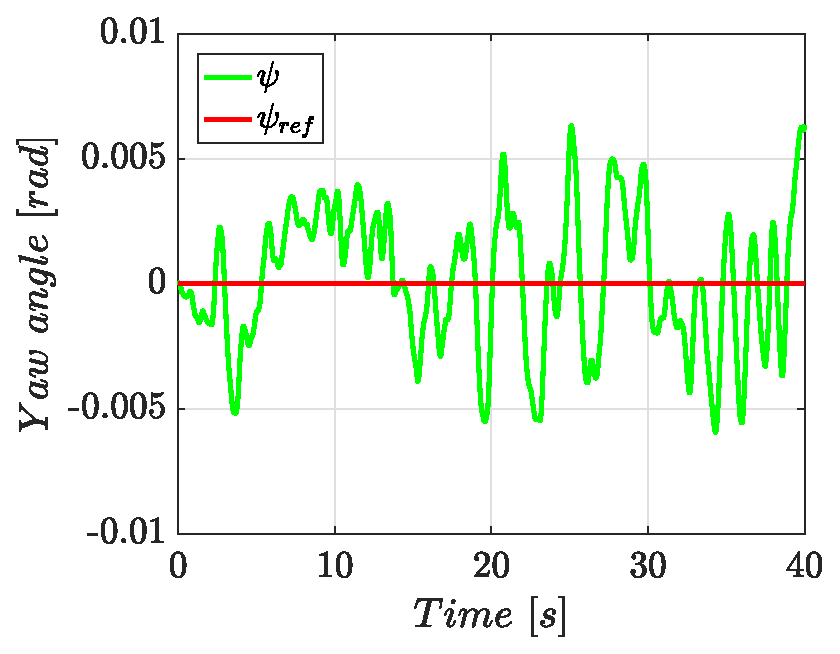
\includegraphics[width=7.0cm]{auto_psi_h_imp}
%\caption{Yaw angle response}
%\label{fig:auto_psi_h_imp}
%\end{subfigure}%
%\begin{subfigure}{.5\linewidth}
%\centering
%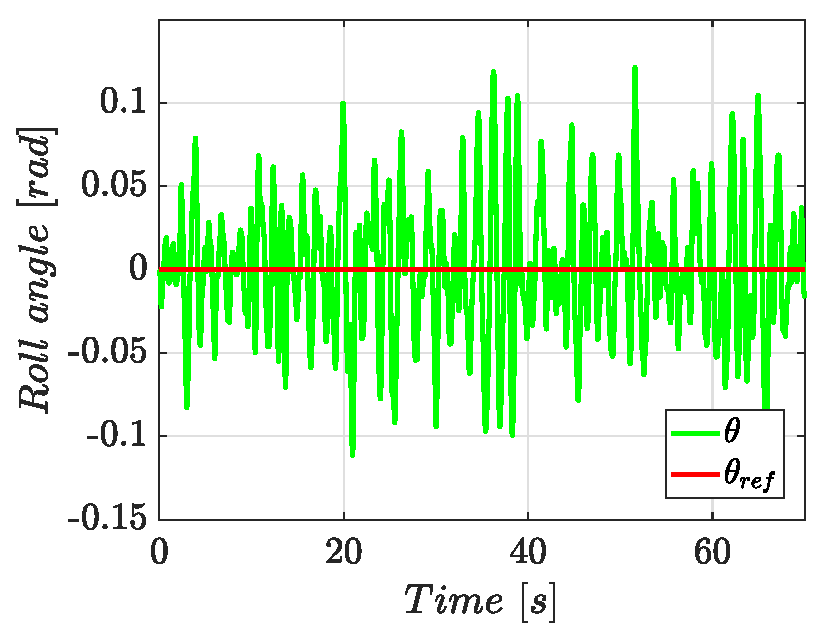
\includegraphics[width=7.0cm]{auto_theta_h_imp}
%\caption{Roll angle response}
%\label{fig:auto_theta_h_imp}
%\end{subfigure}\\[1ex]
%\begin{subfigure}{\linewidth}
%\centering
%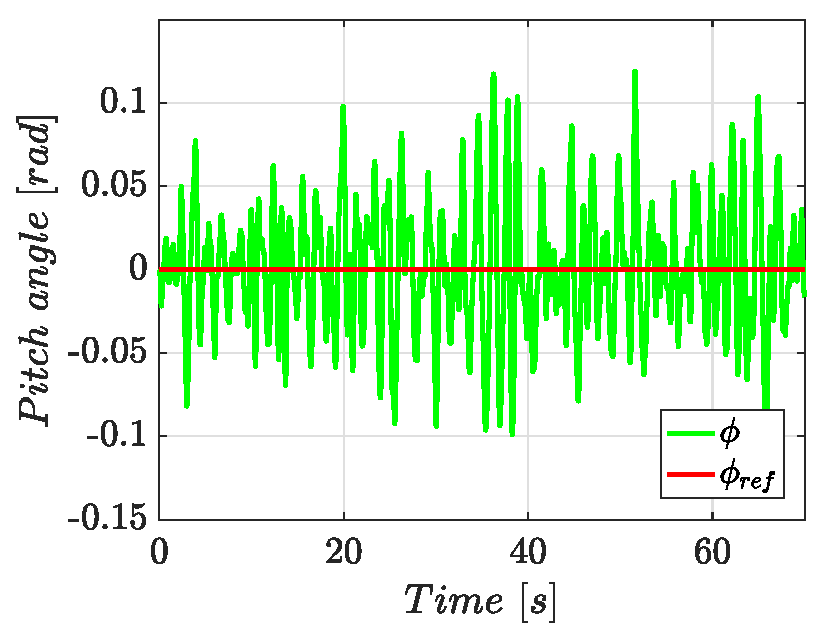
\includegraphics[width=7.0cm]{auto_phi_h_imp}
%\caption{Pitch angle response}
%\label{fig:auto_psi_h_imp}
%\end{subfigure}
%\caption{Attitude response of the GNSS-Dependent modes with a $H_\infty$ controller}
%\label{fig:auto_h_imp}
%\end{figure}


\subsubsection{Performance}

\begin{figure}[h]
\begin{subfigure}{.5\linewidth}
\centering
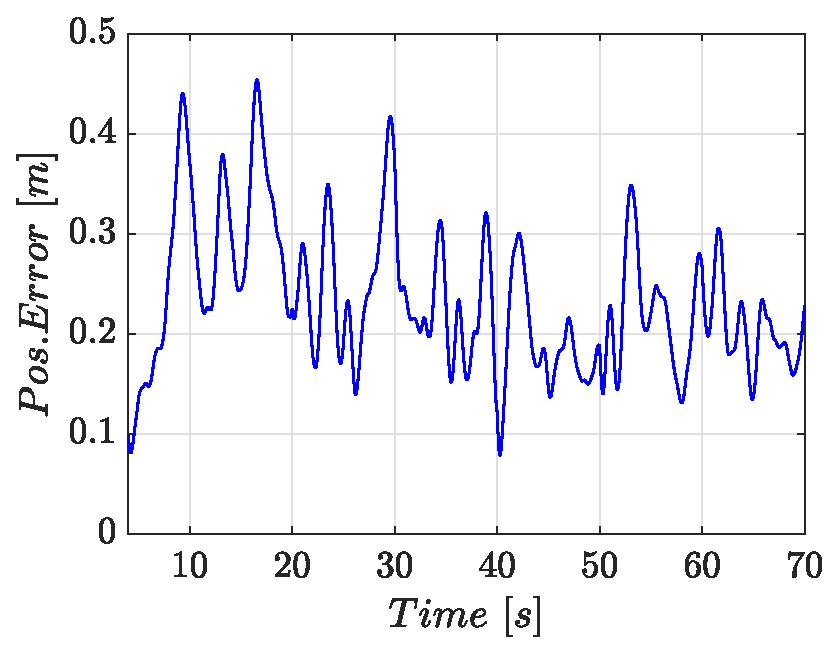
\includegraphics[width=7.0cm]{auto_errorpos_lqi_imp}
\caption{Position error with LQI controller}
\label{fig:auto_errorpos_lqi_imp}
\end{subfigure}%
\begin{subfigure}{.5\linewidth}
\centering
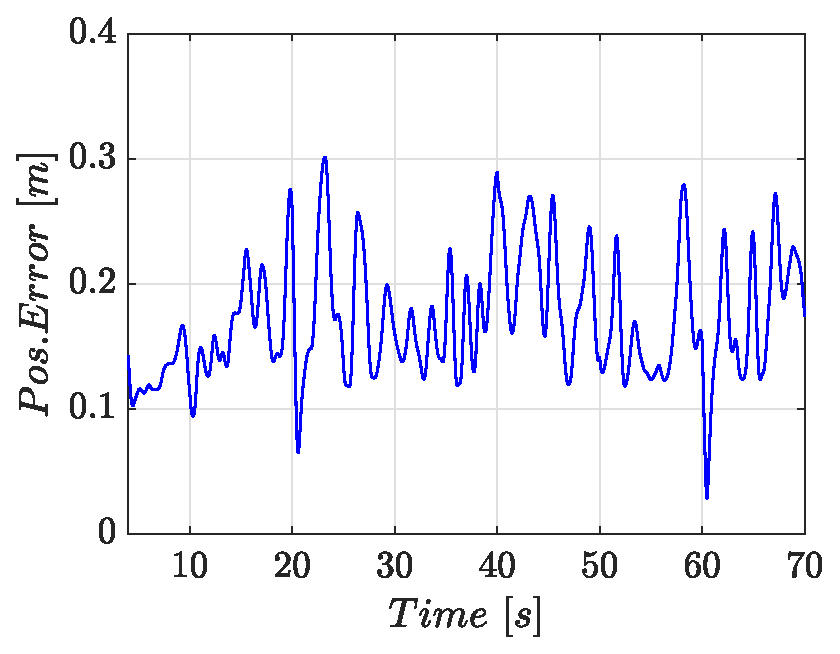
\includegraphics[width=7.0cm]{auto_errorpos_h_imp}
\caption{Position error with $H_\infty$ controller}
\label{fig:auto_errorpos_h_imp}
\end{subfigure}
\caption{Position errors in GNSS-Dependent mode}
\label{fig:auto_errorpos_imp}
\end{figure}



\section{Conclusions}
rgrgrgtrgrtgr
